\documentclass[ignorenonframetext]{beamer}
\usetheme{Darmstadt}
\usecolortheme{beaver}
\usefonttheme{structurebold}
\usepackage{amssymb,amsmath}
\definecolor{links}{HTML}{2A1B81}
\hypersetup{colorlinks,linkcolor=,urlcolor=links}
\usepackage[T1]{fontenc}
\usepackage[utf8]{inputenc}
\usepackage{microtype}
\usepackage{longtable, booktabs}
\usepackage[english]{babel}
\usepackage{pgf, microtype, booktabs, times, etex}
\usepackage{tcolorbox}
\tcbuselibrary{minted,skins}

\newtcblisting{latexcode}{
	listing engine=minted,
	colback=bashcodebg,
	colframe=black!70,
	listing only,
	minted style=colorful,
	minted language=latex,
	minted options={linenos=true,texcl=true},
	left=1mm,
}
\definecolor{bashcodebg}{rgb}{0.85,0.85,0.85}
%\usemintedstyle{emacs}
\beamertemplatenavigationsymbolsempty

\title{\LaTeX{} for Economics and Business Administration}
\author{Thomas de Graaff}
\date{January 12, 2017}

\begin{document}
\frame{\titlepage}

\section{Introduction}\label{introduction}

\subsection{Introduction}\label{introduction-1}

\begin{frame}{Why this workshop?}

\begin{itemize}
\item
  In the \emph{social sciences} few attention to what tools to use (and why)
\item
  \LaTeX{} is used very much in the scientific world and \emph{works} brilliantly together with
  \begin{itemize}
  \item statistical packages, such as \texttt{Stata} and \texttt{R},
  \item markdown/HTML,
  \item reference managers.
  \end{itemize}
  \item Why \emph{I} want to give this workshop
  \begin{itemize}
	  \item intrinsic interest
	  \item my goal: pre-conferences workshops / courses
  \end{itemize}
\end{itemize}
\end{frame}

\begin{frame}{What I want (and don't want) with this workshop}

\begin{itemize}
\item
  Give a general introduction of why some tools work together

  \begin{itemize}
  \item \LaTeX{}
  \item reference managers
  \item (statistical) output
  \end{itemize}
\item
  Give an introduction to \LaTeX{}

  \begin{itemize}
  \item
    First the basics
  \item
    Next workshop: some advanced stuff
  \end{itemize}
\item
  What \emph{I} do not want

  \begin{itemize}
  \item
    Tell you what applications to use (\textbf{you} need to decide and make a \textbf{well-informed} decision)
  \end{itemize}
\end{itemize}

\end{frame}

\texttt{\section{\LaTeX{}}\label{section}

\subsection{Introduction}\label{introduction-2}

\begin{frame}{Background}

\begin{itemize}
	\item \TeX{} has been devised by Donald E. Knuth in the late 70's
	\item \LaTeX{} is a set of macro's around TeX and devised in the 80's
	\item \LaTeX{} is a \emph{typesetting program}, not a \emph{Word processor}

  \begin{itemize}
  \item
    It is actually some code that needs to be compiled
  \item
    Code is typed in by an editor
  \end{itemize}
\item
  So, 
  \begin{itemize}
  \item Huge differences between Word and \LaTeX{}
  \item for \LaTeX{} you need an editor:

    \begin{itemize}
    \item
      Specific editors: TexStudio, TexShop, RStudio
    \item
      General editors: Sublime, TextMate, Notepad++, Vim, Emacs
    \end{itemize}
  \end{itemize}
\end{itemize}

\end{frame}

\subsection{Why \LaTeX{}?}\label{why}

\begin{frame}{Disadvantages}

\begin{itemize}
\item
  Not WYSIWYG
\item
  You nead to learn (quite) some commands

  \begin{itemize}
  \item
    Learning curve, but
  \item
    hurray for
    \href{https://wch.github.io/latexsheet/latexsheet.pdf}{cheat sheets}
    and Google
  \end{itemize}
\item
  Difficult to cooperate with people that went to the \emph{dark side}
\item
  \emph{Basic} \LaTeX{} has \emph{difficulties} with incorporating new
  fonts (Hoefler, minion pro)

  \begin{itemize}
  \item
    XeTeX  \item
    For the purists: \LaTeX{} does it right
    \href{http://oestrem.com/thingstwice/2007/05/latex-vs-word-vs-writer/}{(\LaTeX{}
    vs Word)}
  \end{itemize}
\end{itemize}

\end{frame}

\begin{frame}{Advantages}

\begin{itemize}
\item
  Free (as in beer) and ubiquitous
\item
  WYSIWYM
\item
  Consistent lay-out throughout the whole document (including tables,
  appendices, formulas, source code, etc)
\item
  Internal references are a breeze (references, ToC, ToT \ldots{})
\item
  Forced to structure documents
\item
  Macros, thus scriptable
\item
  Large community, thus a package for almost everything (books,
  articles, presentation, posters, exams, musicscores)
\item
  Superior typography \& output
\item
  Many free \href{https://www.overleaf.com/latex/templates/}{\LaTeX~templates}
\end{itemize}

\end{frame}

\begin{frame}{\LaTeX{} versus Markdown}
	\begin{itemize}
		\item Markdown (all variants): lightweight markup language that can export to \texttt{.doc}, \texttt{.html}, and \texttt{.pdf}.
		\newline
		\item Much easier then \LaTeX{} but less flexible
		\newline
		\item Used by writers/blogs even for complete websites
		\newline
		\item But good interaction with \LaTeX{}; if not only for formula's
	\end{itemize}
\end{frame}

\subsection{Technicalities}\label{technicalities}

\begin{frame}[fragile]{How does \LaTeX{} work in practice?}

\begin{itemize}
\item
  You edit a \texttt{.tex} file without thinking about how it looks

  \begin{itemize}
  \item
    distraction free writing (yeah right)
  \end{itemize}
\item
  You then compile it

  \begin{itemize}
  \item
    \LaTeX{} is unforgiving: if there is an error, usually it does not
    compile
  \item
    Typically, errors are missing brackets or parentheses.
  \end{itemize}
\item
  Typically, source \texttt{.tex} file is compiled into \texttt{.pdf}
\end{itemize}

\end{frame}

\begin{frame}{A process diagram}

\begin{figure}[htbp]
\centering
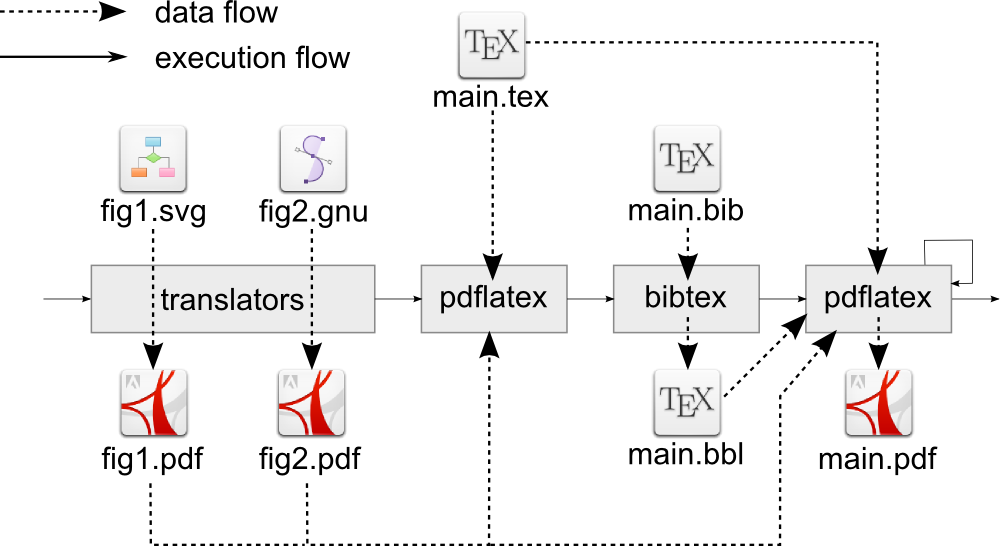
\includegraphics[width=\textwidth]{fig/process.png}
\caption{Process diagram}
\end{figure}

\end{frame}

\begin{frame}[fragile]{Code, documentation and output}

\begin{enumerate}
\def\labelenumi{\arabic{enumi}.}
\item
  Synonyms
\item
  All based on \texttt{.txt} files
\item
  Encompasses almost anything

  \begin{itemize}
  \item
    data itself (\texttt{.csv}, \texttt{.txt})
  \item
    set of commands for data cleaning and statistical analysis
    (\texttt{.do}, \texttt{.R})
  \item
    database with references (\texttt{.bib})
  \item
    text for articles, presentations or websites (\texttt{.tex},
    \texttt{.html})
  \end{itemize}
\item
  Only output is displayed/interpreted differently (e.g., in a browser
  or pdf viewer)
\end{enumerate}

\end{frame}

\subsection{Folder structure and file
names}\label{folder-structure-and-file-names}

\begin{frame}{Folder structure of your new project (theses, paper, assignment \& research)}

\begin{itemize}
\item
  Think \emph{a priori} about project set-up

  \begin{itemize}
  \item
    Seperate analysis, data and output files
  \end{itemize}
\item
  Be careful with source data!

  \begin{itemize}
  \item
    Seperate source and derived data files
  \item
    Typically

    \begin{itemize}
    \item
      you get/collect data
    \item
      transform data
    \item
      analyse data
    \end{itemize}
  \item
    Keep track of all these stages!
  \end{itemize}
\end{itemize}
\end{frame}


\section{TeXstudio}

\subsection{How to work with TeXstudio}

\begin{frame}{A quick tour}
	content...
\end{frame}

\section{Exercises}

\subsection{Baby-steps}

\begin{frame}{First: organize!}
	\begin{enumerate}
		\item Create a specific workshop folder somewhere where you can find it.
		\newline
		\item Think about versioning system and a back-up system
		\newline
		\item E.g.: use dropbox and/or Time Machine 
	\end{enumerate}
\end{frame}

\begin{frame}[fragile]{Document structure: Open from template}
\small
\begin{latexcode}
\documentclass[]{article}
%opening
\title{}
\author{}

\begin{document}
	
	\maketitle
	
	\begin{abstract}
		
	\end{abstract}
	
	\section{}
	
\end{document}
\end{latexcode}
\end{frame}




\end{document}

%%% Local Variables:
%%% mode: latex
%%% TeX-master: t
%%% End:
